\documentclass{article}
\RequirePackage{amsmath}
\RequirePackage{bytefield}
\RequirePackage{graphicx}
\RequirePackage{newtxmath}
\RequirePackage{mathtools}
\RequirePackage{xspace}
\RequirePackage{url}
\RequirePackage{changepage}
\RequirePackage{lmodern}
\RequirePackage[unicode,bookmarksnumbered,bookmarksopen,pdfview=Fit]{hyperref}
\RequirePackage{nameref}
\RequirePackage{enumitem}
\RequirePackage{tabularx}
\RequirePackage{hhline}

\setlength{\oddsidemargin}{-0.25in} % Left margin of 1 in + 0 in = 1 in
\setlength{\textwidth}{7in}   % Right margin of 8.5 in - 1 in - 6.5 in = 1 in
\setlength{\topmargin}{-.75in}  % Top margin of 2 in -0.75 in = 1 in
\setlength{\textheight}{9.2in}  % Lower margin of 11 in - 9 in - 1 in = 1 in
\setlength{\parskip}{1.5ex}
\setlength{\parindent}{0ex}
\renewcommand{\arraystretch}{1.4}
\overfullrule=2cm

\setlist[itemize]{itemsep=0.5ex,topsep=0.2ex,after=\vspace{1.5ex}}

\newcommand{\doctitle}{Zcash Protocol Specification}
\newcommand{\docversion}{Version 2.0-draft-4}
\newcommand{\authors}{Sean Bowe | Daira Hopwood | Taylor Hornby | Nathan Wilcox}

\hypersetup{
  pdfborderstyle={/S/U/W 0.7},
  pdfinfo={
    Title={\doctitle, \docversion},
    Author={\authors}
  }
}

\renewcommand{\sectionautorefname}{\S\!}
\renewcommand{\subsectionautorefname}{\S\!}
\renewcommand{\subsubsectionautorefname}{\S\!}
\newcommand{\crossref}[1]{\autoref{#1} \emph{`\nameref*{#1}\kern -0.1em'} on p.\,\pageref*{#1}}


\mathchardef\mhyphen="2D

\RequirePackage[usenames,dvipsnames]{xcolor}
% https://en.wikibooks.org/wiki/LaTeX/Colors#The_68_standard_colors_known_to_dvips
\newcommand{\eli}[1]{{\color{JungleGreen}\sf{Eli: #1}}}
\newcommand{\sean}[1]{{\color{blue}\sf{Sean: #1}}}
\newcommand{\taylor}[1]{{\color{red}\sf{Taylor: #1}}}
\newcommand{\daira}[1]{{\color{RedOrange}\sf{Daira: #1}}}
\newcommand{\nathan}[1]{{\color{ForestGreen}\sf{Nathan: #1}}}
\newcommand{\todo}[1]{{\color{Sepia}\sf{TODO: #1}}}

\newcommand{\changedcolor}{magenta}
\newcommand{\setchanged}{\color{\changedcolor}}
\newcommand{\changed}[1]{\texorpdfstring{{\setchanged{#1}}}{#1}}

% terminology

\newcommand{\term}[1]{\textsl{#1}\xspace}
\newcommand{\titleterm}[1]{#1\xspace}
\newcommand{\termbf}[1]{\textbf{#1}\xspace}
\newcommand{\conformance}[1]{\textmd{#1}\xspace}

\newcommand{\Zcash}{\termbf{Zcash}}
\newcommand{\Zerocash}{\termbf{Zerocash}}
\newcommand{\Bitcoin}{\termbf{Bitcoin}}
\newcommand{\ZEC}{\termbf{ZEC}}
\newcommand{\zatoshi}{\term{zatoshi}}

\newcommand{\MUST}{\conformance{MUST}}
\newcommand{\MUSTNOT}{\conformance{MUST NOT}}
\newcommand{\SHOULD}{\conformance{SHOULD}}
\newcommand{\SHOULDNOT}{\conformance{SHOULD NOT}}
\newcommand{\MAY}{\conformance{MAY}}

\newcommand{\coin}{\term{note}}
\newcommand{\coins}{\term{notes}}
\newcommand{\Coin}{Note}
\newcommand{\Coins}{Notes}
\newcommand{\coinCommitment}{\term{note commitment}}
\newcommand{\coinCommitments}{\term{note commitments}}
\newcommand{\CoinCommitment}{\titleterm{Note Commitment}}
\newcommand{\CoinCommitments}{\titleterm{Note Commitments}}
\newcommand{\coinCommitmentTree}{\term{note commitment tree}}
\newcommand{\pourDescription}{\term{Xfer description}}
\newcommand{\pourDescriptions}{\term{Xfer descriptions}}
\newcommand{\sequenceOfPourDescriptions}{\changed{sequence of} \pourDescription\changed{\term{s}}\xspace}
\newcommand{\pourTransfer}{\term{Xfer operation}}
\newcommand{\pourTransfers}{\term{Xfer operations}}
\newcommand{\PourTransfer}{\titleterm{Xfer Operation}}
\newcommand{\PourTransfers}{\titleterm{Xfer Operations}}
\newcommand{\fullnode}{\term{full node}}
\newcommand{\fullnodes}{\term{full nodes}}
\newcommand{\anchor}{\term{anchor}}
\newcommand{\anchors}{\term{anchors}}
\newcommand{\block}{\term{block}}
\newcommand{\blocks}{\term{blocks}}
\newcommand{\transaction}{\term{transaction}}
\newcommand{\transactions}{\term{transactions}}
\newcommand{\blockchainview}{\term{blockchain view}}
\newcommand{\mempool}{\term{mempool}}
\newcommand{\treestate}{\term{treestate}}
\newcommand{\treestates}{\term{treestates}}
\newcommand{\serialNumber}{\term{nullifier}}
\newcommand{\serialNumbers}{\term{nullifiers}}
\newcommand{\SerialNumber}{\titleterm{Nullifier}}
\newcommand{\SerialNumbers}{\titleterm{Nullifiers}}
\newcommand{\spentSerials}{\term{nullifier set}}
\newcommand{\SpentSerials}{\titleterm{Nullifier Set}}
% Daira: This doesn't adequately distinguish between zk stuff and transparent stuff
\newcommand{\paymentAddress}{\term{payment address}}
\newcommand{\paymentAddresses}{\term{payment addresses}}
\newcommand{\viewingKey}{\term{viewing key}}
\newcommand{\viewingKeys}{\term{viewing keys}}
\newcommand{\spendingKey}{\term{spending key}}
\newcommand{\spendingKeys}{\term{spending keys}}
\newcommand{\keyTuple}{\term{key tuple}}
\newcommand{\coinPlaintext}{\term{note plaintext}}
\newcommand{\coinPlaintexts}{\term{note plaintexts}}
\newcommand{\CoinPlaintexts}{\titleterm{Note Plaintexts}}
\newcommand{\coinsCiphertext}{\term{transmitted notes ciphertext}}
\newcommand{\authKeypair}{\term{authorization}}
\newcommand{\transmitKeypair}{\term{transmission}}
\newcommand{\discloseKey}{\term{disclosure key}}
\newcommand{\incrementalMerkleTree}{\term{incremental merkle tree}}
\newcommand{\zkSNARK}{\term{zk-SNARK}}
\newcommand{\zkSNARKs}{\term{zk-SNARKs}}
\newcommand{\memo}{\term{memo field}}
\newcommand{\Memos}{\titleterm{Memo Fields}}

% conventions
\newcommand{\bytes}[1]{\underline{\raisebox{-0.22ex}{}\smash{#1}}}
\newcommand{\zeros}[1]{[0]^{#1}}
\newcommand{\hexint}[1]{\mathbf{0x{#1}}}
\newcommand{\dontcare}{\kern -0.06em\raisebox{0.1ex}{\footnotesize{$\times$}}}
\newcommand{\CRH}{\mathsf{CRH}}
\newcommand{\CRHbox}[1]{\CRH\left(\;\raisebox{-1.3ex}{\usebox{#1}}\;\right)}
\newcommand{\FullHash}{\mathtt{SHA256}}
\newcommand{\FullHashbox}[1]{\FullHash\left(\;\raisebox{-1.3ex}{\usebox{#1}}\;\right)}
\newcommand{\Justthebox}[2]{\;\raisebox{#2}{\usebox{#1}}\;}
\newcommand{\setof}[1]{\{{#1}\}}

% key pairs:
\newcommand{\PaymentAddress}{\mathsf{addr_{pk}}}
\newcommand{\SpendingKey}{\mathsf{addr_{sk}}}
\newcommand{\PaymentAddressLeadByte}{\hexint{92}}
\newcommand{\SpendingKeyLeadByte}{\hexint{??}}
\newcommand{\CoinCommitmentLeadByte}{\hexint{C0}}
\newcommand{\AuthPublic}{\mathsf{a_{pk}}}
\newcommand{\AuthPrivate}{\mathsf{a_{sk}}}
\newcommand{\AuthPublicOld}[1]{\mathsf{a^{old}_{pk,\mathnormal{#1}}}}
\newcommand{\AuthPrivateOld}[1]{\mathsf{a^{old}_{sk,\mathnormal{#1}}}}
\newcommand{\AuthPublicNew}[1]{\mathsf{a^{new}_{pk,\mathnormal{#1}}}}
\newcommand{\AuthPrivateNew}[1]{\mathsf{a^{new}_{sk,\mathnormal{#1}}}}
\newcommand{\AddressPublicNew}[1]{\mathsf{addr^{new}_{pk,\mathnormal{#1}}}}
\newcommand{\enc}{\mathsf{enc}}
\newcommand{\disclose}{\mathsf{disclose}}
\newcommand{\shared}{\mathsf{shared}}
\newcommand{\DHSecret}[1]{\mathsf{dhsecret}_{#1}}
\newcommand{\DHSecretCompare}[1]{\mathsf{dhsecret}^*_{#1}}
\newcommand{\EphemeralPublic}{\mathsf{epk}}
\newcommand{\EphemeralPublicCompare}{\mathsf{epk}^*}
\newcommand{\EphemeralPrivate}{\mathsf{esk}}
\newcommand{\EphemeralPrivateClamped}{\mathsf{esk_{clamped}}}
\newcommand{\TransmitPublic}{\mathsf{pk_{enc}}}
\newcommand{\TransmitPublicNew}[1]{\mathsf{pk^{new}_{\enc,\mathnormal{#1}}}}
\newcommand{\TransmitPrivate}{\mathsf{sk_{enc}}}
\newcommand{\Value}{\mathsf{v}}
\newcommand{\ValueNew}[1]{\mathsf{v^{new}_\mathnormal{#1}}}

% Coins
\newcommand{\CoinTuple}[1]{\mathbf{n}_{#1}}
\newcommand{\CoinPlaintext}[1]{\mathbf{np}_{#1}}
\newcommand{\CoinCommitRand}{\mathsf{r}}
\newcommand{\CoinCommitRandOld}[1]{\mathsf{r^{old}_\mathnormal{#1}}}
\newcommand{\CoinCommitRandNew}[1]{\mathsf{r^{new}_\mathnormal{#1}}}
\newcommand{\CoinAddressRand}{\mathsf{\uprho}}
\newcommand{\CoinAddressRandOld}[1]{\mathsf{\uprho^{old}_\mathnormal{#1}}}
\newcommand{\CoinAddressRandNew}[1]{\mathsf{\uprho^{new}_\mathnormal{#1}}}
\newcommand{\CoinAddressPreRand}{\mathsf{\upvarphi}}
\newcommand{\CoinCommitS}{\mathsf{s}}
\newcommand{\sn}{\mathsf{nf}}
\newcommand{\snOld}[1]{\sn^\mathsf{old}_\mathnormal{#1}}
\newcommand{\hSigInputVersionByte}{\hexint{C1}}
\newcommand{\Memo}{\mathsf{memo}}
\newcommand{\CurveMultiply}{\mathsf{Curve25519}}
\newcommand{\CurveBase}{\bytes{9}}
\newcommand{\DecryptNote}{\mathtt{DecryptNote}}
\newcommand{\Plaintext}{\mathbf{P}}
\newcommand{\Ciphertext}{\mathbf{C}}
\newcommand{\Key}{\mathsf{K}}
\newcommand{\TransmitPlaintext}[1]{\Plaintext^\enc_{#1}}
\newcommand{\TransmitCiphertext}[1]{\Ciphertext^\enc_{#1}}
\newcommand{\TransmitKey}[1]{\Key^\enc_{#1}}
\newcommand{\TransmitKeyCompare}[1]{\Key^*_{#1}}
\newcommand{\DerivedKey}[1]{\Key^\disclose_{#1}}
\newcommand{\DisclosePlaintext}[1]{\Plaintext^\disclose_{#1}}
\newcommand{\DiscloseCiphertext}[1]{\Ciphertext^\disclose_{#1}}
\newcommand{\SharedPlaintext}{\Plaintext^\shared}
\newcommand{\KDF}{\mathsf{KDF}}
\newcommand{\KDFLeadByte}{\hexint{C2}}
\newcommand{\SymEncrypt}[1]{\mathsf{SymEncrypt}_{#1}}
\newcommand{\SymDecrypt}[1]{\mathsf{SymDecrypt}_{#1}}
\newcommand{\SymSpecific}{\mathsf{AEAD\_CHACHA20\_POLY1305}}
\newcommand{\SymCipher}{\mathsf{ChaCha20}}
\newcommand{\SymAuth}{\mathsf{Poly1305}}
\newcommand{\Clamp}{\mathsf{clamp_{Curve25519}}}
\newcommand{\PRF}[2]{\mathsf{{PRF}^{#2}_\mathnormal{#1}}}
\newcommand{\PRFaddr}[1]{\PRF{#1}{addr}}
\newcommand{\PRFsn}[1]{\PRF{#1}{\sn}}
\newcommand{\PRFpk}[1]{\PRF{#1}{pk}}
\newcommand{\PRFrho}[1]{\PRF{#1}{\CoinAddressRand}}
\newcommand{\PRFdk}[1]{\PRF{#1}{dk}}
\newcommand{\SHA}{\mathtt{SHA256Compress}}
\newcommand{\SHAName}{\term{SHA-256 compression}}
\newcommand{\SHAOrig}{\term{SHA-256}}
\newcommand{\cm}{\mathsf{cm}}
\newcommand{\cmNew}[1]{\mathsf{{cm}^{new}_\mathnormal{#1}}}
\newcommand{\ReplacementCharacter}{\textsf{U+FFFD}}
\newcommand{\CryptoBoxSeal}{\mathsf{crypto\_box\_seal}}
\newcommand{\ECDSAr}{\mathsf{r}}
\newcommand{\ECDSAs}{\mathsf{s}}

% merkle tree
\newcommand{\MerkleDepth}{\mathsf{d}}

% bitcoin
\newcommand{\vin}{\mathtt{vin}}
\newcommand{\vout}{\mathtt{vout}}
\newcommand{\npour}{\mathtt{nxfer}}
\newcommand{\vpour}{\mathtt{vxfer}}
\newcommand{\vpubOldField}{\mathtt{vpub\_old}}
\newcommand{\vpubNewField}{\mathtt{vpub\_new}}
\newcommand{\vsum}[2]{\smashoperator[r]{\sum_{#1}^{#2}}}
\newcommand{\anchorField}{\mathtt{anchor}}
\newcommand{\pourSig}{\mathtt{xferSig}}
\newcommand{\pourPubKey}{\mathtt{xferPubKey}}
\newcommand{\dataToBeSigned}{\mathtt{dataToBeSigned}}
\newcommand{\serials}{\mathtt{nullifiers}}
\newcommand{\commitments}{\mathtt{commitments}}
\newcommand{\ephemeralKey}{\mathtt{ephemeralKey}}
\newcommand{\encCiphertexts}{\mathtt{encCiphertexts}}
\newcommand{\discloseCiphertexts}{\mathtt{discloseCiphertexts}}
\newcommand{\randomSeed}{\mathtt{randomSeed}}
\newcommand{\rt}{\mathsf{rt}}
\newcommand{\Varies}{\textit{Varies}}
\newcommand{\heading}[1]{\multicolumn{1}{c|}{#1}}
\newcommand{\type}[1]{\texttt{#1}}

% xfer
\newcommand{\hSig}{\mathsf{h_{Sig}}}
\newcommand{\hSigText}{\texorpdfstring{$\hSig$}{hSig}}
\newcommand{\h}[1]{\mathsf{h_{\mathnormal{#1}}}}
\newcommand{\NOld}{\mathrm{N}^\mathsf{old}}
\newcommand{\NNew}{\mathrm{N}^\mathsf{new}}
\newcommand{\allN}[1]{\mathrm{1}..\mathrm{N}^\mathsf{#1}}
\newcommand{\allOld}{\allN{old}}
\newcommand{\allNew}{\allN{new}}
\newcommand{\setofOld}{\setof{\allOld}}
\newcommand{\setofNew}{\setof{\allNew}}
\newcommand{\vmacs}{\mathtt{vmacs}}
\newcommand{\zkproofSize}{\mathtt{zkproofSize}}
\newcommand{\zkproof}{\mathtt{zkproof}}
\newcommand{\PourCircuit}{\term{\texttt{Xfer} circuit}}
\newcommand{\PourStatement}{\texttt{Xfer}}
\newcommand{\PourProof}{\pi_{\PourStatement}}
\newcommand{\vpubOld}{\mathsf{v_{pub}^{old}}}
\newcommand{\vpubNew}{\mathsf{v_{pub}^{new}}}
\newcommand{\cOld}[1]{\mathbf{n}_{#1}^\mathsf{old}}
\newcommand{\cNew}[1]{\mathbf{n}_{#1}^\mathsf{new}}
\newcommand{\cpNew}[1]{\mathbf{np}_{#1}^\mathsf{new}}
\newcommand{\vOld}[1]{\mathsf{v}_{#1}^\mathsf{old}}
\newcommand{\vNew}[1]{\mathsf{v}_{#1}^\mathsf{new}}
\newcommand{\NP}{\mathsf{NP}}
\newcommand{\treepath}[1]{\mathsf{path}_{#1}}
\newcommand{\COMM}[1]{\mathsf{COMM}_{#1}}
\newcommand{\COMMtrapdoor}{\term{\textsf{COMM} trapdoor}}
\newcommand{\Commitment}{\mathtt{NoteCommitment}}
\newcommand{\Receive}{\mathsf{Receive}}


\begin{document}

\title{\doctitle \\
\Large \docversion}
\author{\authors}
\date{\today}
\maketitle

\tableofcontents
\newpage


\section{Introduction}

\Zcash is an implementation of the \term{Decentralized Anonymous Payment}
scheme \Zerocash \cite{ZerocashOakland} with some adjustments to terminology,
functionality and performance. It bridges the existing \emph{transparent}
payment scheme used by \Bitcoin with a \emph{confidential} payment scheme
protected by zero-knowledge succinct non-interactive arguments of knowledge
(\zkSNARKs).

Changes from the original \Zerocash are highlighted in \changed{\changedcolor}.


\section{Caution}

\Zcash security depends on consensus. Should your program diverge from
consensus, its security is weakened or destroyed. The cause of the divergence
doesn't matter: it could be a bug in your program, it could be an error in
this documentation which you implemented as described, or it could be you do
everything right but other software on the network behaves unexpectedly. The
specific cause will not matter to the users of your software whose wealth is
lost.

Having said that, a specification of \emph{intended} behaviour is essential
for security analysis, understanding of the protocol, and maintenance of
Zcash Core and related software. If you find any mistake in this specification,
please contact \texttt{<security@z.cash>}. While the production \Zcash network
has yet to be launched, please feel free to do so in public even if you believe
the mistake may indicate a security weakness.


\section{Conventions}

\subsection{Integers, Bit Sequences, and Endianness}

All integers in \emph{\Zcash-specific} encodings are unsigned, have a fixed
bit length, and are encoded as big-endian. \changed{The definition of
the encryption scheme based on $\SymSpecific$ \cite{rfc7539} in \crossref{inband}
uses length fields encoded as little-endian. Also, Curve25519 public and
private keys are defined as byte sequences, which are converted from integers
using little-endian encoding.}

The notation $\hexint{}$ followed by a string of \textbf{boldface} hexadecimal
digits represents the corresponding integer converted from hexadecimal.

In bit layout diagrams, each box of the diagram represents a sequence of bits.
The bit length is given explicitly in each box, except for the case of a single
bit, or for the notation $\zeros{n}$ which represents the sequence of $n$ zero bits.
If the content of the box is a byte sequence, it is implicitly converted to
a sequence of bits using big-endian order. The bit sequences are then
concatenated in the order shown from left to right, and the result is converted
to a sequence of bytes, again using big-endian order.

\newsavebox{\examplebox}
\begin{lrbox}{\examplebox}
\setchanged
\begin{bytefield}[bitwidth=0.6em]{32}
        \bitbox{2}{0} &
        \bitbox{2}{1} &
        \bitbox{2}{0} &
        \bitbox{2}{0} &
        \bitbox{16}{16 bit $\hexint{ABCD}$} &
        \bitbox{12}{12 bit $\hexint{0123}$} &
\end{bytefield}
\end{lrbox}

For example, the diagram
\begin{itemize}
  \item[] $\Justthebox{\examplebox}{-1.3ex}$
\end{itemize}

represents the byte sequence $[\hexint{4A}, \hexint{BC}, \hexint{D1}, \hexint{23}]$.

The notation $\allN{}$, used as a subscript, means the sequence of values
with indices $1$ through $\mathrm{N}$ inclusive. For example,
$\AuthPublicNew{\allNew}$ means the sequence $[\AuthPublicNew{\mathrm{1}},
\AuthPublicNew{\mathrm{2}}, ...\;\AuthPublicNew{\NNew}]$.

The symbol $\bot$ is used to indicate unavailable information or a failed decryption.

\subsection{Cryptographic Functions}

$\CRH$ is a collision-resistant hash function. In \Zcash, the $\SHAName$ function
is used which takes a 512-bit block and produces a 256-bit hash. This is
different from the $\SHAOrig$ function, which hashes arbitrary-length sequences.
\cite{sha256}

$\PRF{x}{}$ is a pseudo-random function seeded by $x$. \changed{Four} \emph{independent}
$\PRF{x}{}$ are needed in our scheme: $\PRFaddr{x}$, $\PRFsn{x}$, $\PRFpk{x}$\changed{,
and $\PRFrho{x}$}.

It is required that $\PRFsn{x}$ \changed{and $\PRFrho{x}$} be collision-resistant
across all $x$ --- i.e. it should not be feasible to find $(x, y) \neq (x', y')$
such that $\PRFsn{x}(y) = \PRFsn{x'}(y')$\changed{, and similarly for $\PRFrho{}$}.

In \Zcash, the $\SHAName$ function is used to construct all of these
functions.

\newcommand{\iminusone}{\hspace{0.3pt}\scriptsize{$i$\hspace{0.6pt}-1}}

\newsavebox{\addrbox}
\begin{lrbox}{\addrbox}
\setchanged
\begin{bytefield}[bitwidth=0.06em]{512}
        \bitbox{18}{0} &
        \bitbox{18}{0} &
        \bitbox{18}{0} &
        \bitbox{18}{0} &
        \bitbox{224}{252 bit $x$} &
        \bitbox{200}{$\zeros{253}$} &
        \bitbox{56}{3 bit $t$} &
\end{bytefield}
\end{lrbox}

\newsavebox{\snbox}
\begin{lrbox}{\snbox}
\setchanged
\begin{bytefield}[bitwidth=0.06em]{512}
        \bitbox{18}{0} &
        \bitbox{18}{1} &
        \bitbox{18}{0} &
        \bitbox{18}{0} &
        \bitbox{224}{252 bit $\AuthPrivate$} &
        \bitbox{256}{256 bit $\CoinAddressRand$} &
\end{bytefield}
\end{lrbox}

\newsavebox{\pkbox}
\begin{lrbox}{\pkbox}
\setchanged
\begin{bytefield}[bitwidth=0.06em]{512}
        \bitbox{18}{0} &
        \bitbox{18}{\iminusone} &
        \bitbox{18}{0} &
        \bitbox{18}{1} &
        \bitbox{224}{252 bit $\AuthPrivate$} &
        \bitbox{256}{256 bit $\hSig$}
\end{bytefield}
\end{lrbox}

\newsavebox{\rhobox}
\begin{lrbox}{\rhobox}
\setchanged
\begin{bytefield}[bitwidth=0.06em]{512}
        \bitbox{18}{0} &
        \bitbox{18}{\iminusone} &
        \bitbox{18}{1} &
        \bitbox{18}{0} &
        \bitbox{224}{252 bit $\CoinAddressPreRand$} &
        \bitbox{256}{256 bit $\hSig$}
\end{bytefield}
\end{lrbox}

\begin{equation*}
\begin{aligned}
&\setchanged \PRFaddr{x}(t) &\setchanged := \CRHbox{\addrbox} \\
\sn =\;& \PRFsn{\AuthPrivate}(\CoinAddressRand) &:= \CRHbox{\snbox} \\
\h{i} =\;& \PRFpk{\AuthPrivate}(i, \hSig) &:= \CRHbox{\pkbox} \\
\setchanged \CoinAddressRandNew{i} =\;&\setchanged \PRFrho{\CoinAddressPreRand}(i, \hSig)
&\setchanged := \CRHbox{\rhobox}
\end{aligned}
\end{equation*}

\changed{
\subparagraph{Note:}
The most significant four bits of the first byte are used to distinguish
different uses of $\CRH$, ensuring that the functions are independent.
In addition to the inputs shown here, the first four bits $\mathtt{1100}$
(i.e. a first byte of \textbf{0xC\dontcare}) are used to distinguish uses
of the full $\SHAOrig$ hash function -- see \crossref{comm} and \crossref{hsig}.
}


\section{Concepts}

\subsection{Payment Addresses and Spending Keys}

A \keyTuple $(\SpendingKey, \PaymentAddress)$ is
generated by users who wish to receive payments under this scheme.
The \paymentAddress $\PaymentAddress$ is derived from the \spendingKey
$\SpendingKey$.

The following diagram depicts the relations between key components.
Arrows point from a component to any other component(s) that can be derived
from it.

\begin{center}
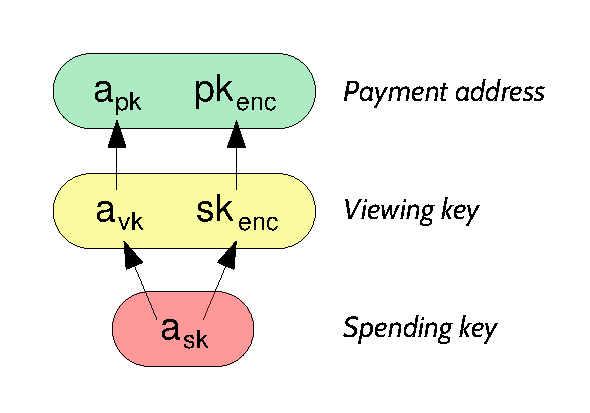
\includegraphics[scale=.8]{key_components}
\end{center}

The composition of \paymentAddresses and \spendingKeys
is a cryptographic protocol detail that should not normally be
exposed to users. However, user-visible operations should be provided
to obtain a \paymentAddress or \viewingKey from a \spendingKey.

\changed{$\AuthPrivate$ is 252 bits.}
$\AuthPublic$, $\TransmitPrivate$, and $\TransmitPublic$, are each 256 bits.

\changed{$\AuthPublic$, $\TransmitPrivate$ and $\TransmitPublic$ are derived
as follows:}
{\hfuzz=50pt
\begin{equation*}
\begin{aligned}
\AuthPublic &:= \changed{\PRFaddr{\AuthPrivate}(0)} \\
\TransmitPrivate &:= \changed{\Clamp(\PRFaddr{\AuthPrivate}(1))} \\
\TransmitPublic &:= \changed{\CurveMultiply(\TransmitPrivate, \CurveBase)}
\end{aligned}
\end{equation*}
}

\changed{
where
\begin{itemize}
  \item $\CurveMultiply(\bytes{n}, \bytes{q})$ performs point
multiplication of the Curve25519 public key represented by the byte
sequence $\bytes{q}$ by the Curve25519 secret key represented by the
byte sequence $\bytes{n}$, as defined in section 2 of \cite{Curve25519};
  \item $\CurveBase$ is the public byte sequence representing the Curve25519
base point;
  \item $\Clamp(\bytes{x})$ takes a 32-byte sequence $\bytes{x}$ as input
and returns a byte sequence representing a Curve25519 private key, with
bits ``clamped'' as described in section 3 of \cite{Curve25519}:
``clear bits 0, 1, 2 of the first byte, clear bit 7 of the last byte,
and set bit 6 of the last byte.'' Here the bits of a byte are numbered
such that bit $b$ has numeric weight $2^b$.
\end{itemize}
}

Users can accept payment from multiple parties with a single
$\PaymentAddress$ and the fact that these payments are destined to
the same payee is not revealed on the blockchain, even to the
paying parties. \emph{However} if two parties collude to compare a
$\PaymentAddress$ they can trivially determine they are the same. In the
case that a payee wishes to prevent this they should create a distinct
\paymentAddress for each payer.

\subsection{\Coins}

A \coin (denoted $\CoinTuple{}$) is a tuple $\changed{(\AuthPublic, \Value,
\CoinAddressRand, \CoinCommitRand)}$ which represents that a value $\Value$ is
spendable by the recipient who holds the \spendingKey $\AuthPrivate$ corresponding
to $\AuthPublic$, as described in the previous section.
 
\begin{itemize}
    \item $\AuthPublic$ is a 32-byte \authKeypair public key of the recipient.
    \item $\Value$ is a 64-bit unsigned integer representing the value of the
        \coin in \zatoshi (1 \ZEC = $10^8$ \zatoshi).
    \item $\CoinAddressRand$ is a 32-byte $\PRFsn{\AuthPrivate}$ preimage.
    \item $\CoinCommitRand$ is a 24-byte \COMMtrapdoor.
\end{itemize}

$\CoinCommitRand$ is randomly generated by the sender. \changed{$\CoinAddressRand$
is generated from a random seed $\CoinAddressPreRand$ using
$\PRFrho{\CoinAddressPreRand}$.} Only a commitment to these values is disclosed
publicly, which allows the tokens $\CoinCommitRand$ and $\CoinAddressRand$ to blind
the value and recipient \emph{except} to those who possess these tokens.

\subsubsection{\CoinCommitments} \label{comm}

The underlying $\Value$ and $\AuthPublic$ are blinded with $\CoinAddressRand$
and $\CoinCommitRand$ using the collision-resistant hash function \changed{$\FullHash$}.
The resulting hash $\cm = \Commitment(\CoinTuple{})$.

\newsavebox{\cmbox}
\begin{lrbox}{\cmbox}
\setchanged
\begin{bytefield}[bitwidth=0.042em]{776}
        \bitbox{128}{8 bit $\CoinCommitmentLeadByte$} &
	\bitbox{256}{256 bit $\AuthPublic$} &
	\bitbox{128}{64 bit $\Value$} &
	\bitbox{256}{256 bit $\CoinAddressRand$}
	\bitbox{192}{192 bit $\CoinCommitRand$} &
\end{bytefield}
\end{lrbox}

\changed{
\hskip 1.5em $\cm := \FullHashbox{\cmbox}$
}

\subsubsection{\SerialNumbers}

A \serialNumber (denoted $\sn$) is derived from the $\CoinAddressRand$ component
of a \coin as $\PRFsn{\AuthPrivate}(\CoinAddressRand)$. A \coin is spent by proving
knowledge of $\CoinAddressRand$ and $\AuthPrivate$ in zero knowledge while
disclosing its \serialNumber $\sn$, allowing $\sn$ to be used to prevent double-spending.

\subsubsection{\CoinPlaintexts and \Memos} \label{coinpt}

Transmitted \coins are stored on the blockchain in encrypted form, together with
a \coinCommitment $\cm$.

The \coinPlaintexts associated with a \pourDescription are encrypted to the
respective \transmitKeypair keys $\TransmitPublicNew{\allNew}$,
and the result forms part of a \coinsCiphertext (see \crossref{inband}
for further details).

Each \coinPlaintext (denoted $\CoinPlaintext{}$) consists of
$(\changed{\AuthPublic,\;}\Value, \CoinAddressRand, \CoinCommitRand\changed{, \Memo})$.

The first \changed{four} of these fields are as defined earlier.
\changed{$\Memo$ is a 64-byte \memo associated with this \coin.

The usage of the $\memo$ is by agreement between the sender and recipient of the
\coin. It should be encoded as a UTF-8 human-readable string \cite{Unicode}, padded
with zero bytes. Wallet software is expected to strip any trailing zero bytes and
then display the resulting UTF-8 string to the recipient user, where applicable.
Incorrect UTF-8-encoded byte sequences should be displayed as replacement characters
(\ReplacementCharacter). This does not preclude uses of the \memo by automated
software, but specification of such usage is not in the scope of this document.
}

The encoding of a \coinPlaintext consists of, in order:
\begin{equation*}
\begin{bytefield}[bitwidth=0.035em]{1288}
\changed{
    \bitbox{256}{$\AuthPublic$ (32 bytes)}&
  &}\bitbox{168}{$\Value$ (8 bytes)} &
    \bitbox{256}{$\CoinAddressRand$ (32 bytes)} &
    \bitbox{192}{$\CoinCommitRand$ (\changed{24} bytes)} &
    \changed{\bitbox{512}{$\Memo$ (64 bytes)}}
\end{bytefield}
\end{equation*}

\begin{itemize}
\changed{
    \item 32 bytes specifying $\AuthPublic$.
}
    \item 8 bytes specifying a big-endian encoding of $\Value$.
    \item 32 bytes specifying $\CoinAddressRand$.
    \item \changed{24} bytes specifying $\CoinCommitRand$.
\changed{
    \item 64 bytes specifying $\Memo$.
}
\end{itemize}


\subsection{\CoinCommitment Tree}

\begin{center}
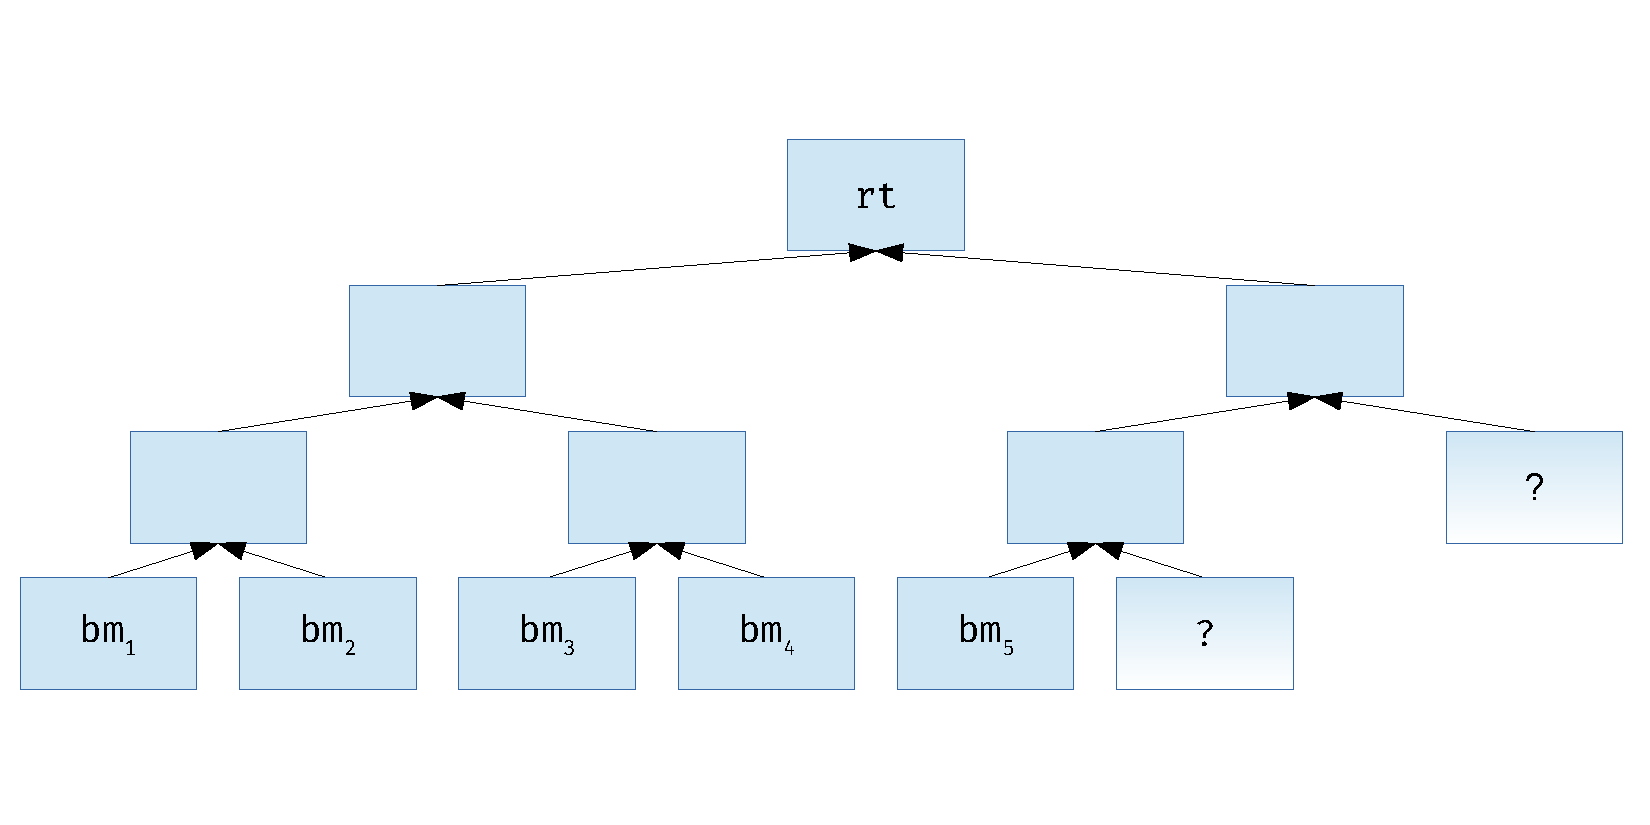
\includegraphics[scale=.4]{incremental_merkle}
\end{center}

The \coinCommitmentTree is an \incrementalMerkleTree of depth $\MerkleDepth$ used to
store \coinCommitments that \pourTransfers produce. Just as the \term{unspent
transaction output set} (UTXO) used in Bitcoin, it is used to express the existence
of value and the capability to spend it. However, unlike the UTXO, it is \emph{not}
the job of this tree to protect against double-spending, as it is append-only.

Blocks in the blockchain are associated (by all nodes) with the root of this tree
after all of its constituent \pourDescriptions' \coinCommitments have been
entered into the tree associated with the previous block.

\subsection{\SpentSerials}

Transactions insert \serialNumbers into a \spentSerials which is maintained
alongside the UTXO by all nodes.

\eli{a tx is just a string, so it doesn't insert anything. Rather, nodes process 
tx's and the ``good'' ones lead to the addition of \serialNumbers to the
\spentSerials.}

Transactions that attempt to insert a \serialNumber into this set that already
exists within it are invalid as they are attempting to double-spend.

\eli{After defining \term{transaction}, one should define what a \term{legal tx} is
(this definition depends on a particular blockchain [view]) and only then can one
talk about ``attempts'' of transactions, and insertions of \serialNumbers into the
\spentSerials.}

\subsection{The Blockchain}

At a given point in time, the \blockchainview of each \fullnode consists of a
sequence of one or more valid \blocks. Each \block consists of a sequence of one or
more \transactions. In a given node's \blockchainview, \treestates are chained in an
obvious way:

\begin{itemize}
  \item The input \treestate of the first \block is the empty \treestate.
  \item The input \treestate of the first \transaction of a \block is the final
        \treestate of the immediately preceding \block.
  \item The input \treestate of each subsequent \transaction in a \block is the
        output \treestate of the immediately preceding \transaction.
  \item The final \treestate of a \block is the output \treestate of its last
        \transaction.
\end{itemize}

An \anchor is a Merkle tree root of a \treestate, and uniquely identifies that
\treestate given the assumed security properties of the Merkle tree's hash function.

Each \transaction is associated with a \sequenceOfPourDescriptions.
\todo{They also have a transparent value flow that interacts with the Pour
\changed{$\vpubOld$ and} $\vpubNew$.}
Inputs and outputs are associated with a value.

The total value of the outputs must not exceed the total value of the inputs.

The \anchor of the \changed{first} \pourDescription in a \transaction must refer to
some earlier \block's final \treestate.

\changed{
The \anchor of each subsequent \pourDescription may refer either to some earlier
\block's final \treestate, or to the output \treestate of the immediately preceding
\pourDescription.
}

These conditions act as constraints on the blocks that a \fullnode will
accept into its \blockchainview.

We rely on Bitcoin-style consensus for \fullnodes to eventually converge on their 
views of valid \blocks, and therefore of the sequence of \treestates in those 
\blocks.


\subparagraph{Value pool}

Transaction inputs insert value into a \term{value pool}, and transaction outputs 
remove value from this pool. The remaining value in the pool is available to miners 
as a fee.

\section{\PourTransfers and Descriptions} \label{pourdesc}

A \pourDescription is data included in a \block that describes a \pourTransfer,
i.e. a confidential value transfer. This kind of value transfer is the primary
\Zcash-specific operation performed by transactions; it uses, but should not be
confused with, the \PourCircuit used for the \zkSNARK proof and verification.

A \pourTransfer spends $\NOld$ \coins $\cOld{\allOld}$ and transparent input
$\vpubOld$, and creates $\NNew$ \coins $\cNew{\allNew}$ and transparent output
$\vpubNew$.

\changed{
\Zcash transactions have the following additional fields:

\begin{center}
\begin{tabularx}{0.9\textwidth}{|c|l|l|X|}
\hline
Bytes & \heading{Name} & \heading{Data Type} & \heading{Description} \\
\hhline{|=|=|=|=|}

\Varies & $\npour$ & \type{compactSize uint} & The number of \pourDescriptions (i.e.
items in $\vpour$). \\ \hline

$880 \times \npour$ & $\vpour$ & \type{XferDescription[$\npour$]} & The \sequenceOfPourDescriptions in
this \transaction. \\ \hline

33 & $\pourPubKey$ & \type{char[33]} & An encoding of a ECDSA public verification key,
using the secp256k1 curve and parameters defined in \cite{sec2-ecdsa} and
\cite{secp256k1}. \\ \hline

64 & $\pourSig$ & \type{char[64]} & A signature on part of the \transaction encoding,
to be verified using $\pourPubKey$. \\ \hline
\end{tabularx}
\end{center}

The encoding of $\pourPubKey$ and the data to be signed are specified in
more detail in \crossref{nonmalleability}.
}

Each \type{XferDescription} consists of:

\begin{center}
\begin{tabularx}{0.9\textwidth}{|c|l|l|X|}
\hline
Bytes & \heading{Name} & \heading{Data Type} & \heading{Description} \\
\hhline{|=|=|=|=|}

\setchanged 8 &\setchanged $\vpubOldField$ &\setchanged \type{int64\_t} &\mbox{}\setchanged
A value $\vpubOld$ that the \PourTransfer removes from the value pool. \\ \hline

8 & $\vpubNewField$ & \type{int64\_t} & A value $\vpubNew$ that the \PourTransfer inserts
into the value pool. \\ \hline

32 & $\anchorField$ & \type{char[32]} & A merkle root $\rt$ of the \coinCommitmentTree at
some block height in the past, or the merkle root produced by a previous \pourTransfer in
this transaction. \sean{We need to be more specific here.} \\ \hline

64 & $\serials$ & \type{char[32][$\NOld$]} & A sequence of \serialNumbers of the input
\coins $\snOld{\allOld}$. \\ \hline

64 & $\commitments$ & \type{char[32][$\NNew$]}. & A sequence of \coinCommitments for the
output \coins $\cmNew{\allNew}$. \\ \hline

32 & $\ephemeralKey$ & \type{char[32]} & A Curve25519 public key $\EphemeralPublic$. \\ \hline

288 & $\encCiphertexts$ & \type{char[144][$\NNew$]} & A sequence of ciphertext
components for the encrypted output \coins, $\TransmitCiphertext{\allNew}$. \\ \hline

\setchanged 32 &\setchanged $\randomSeed$ &\setchanged \type{char[32]} &\mbox{}\setchanged
A 256-bit seed that must be chosen independently at random for each \pourDescription. \\ \hline

64 & $\vmacs$ & \type{char[32][$\NOld$]} & A sequence of message authentication tags
$\h{\allOld}$ that bind $\hSig$ to each $\AuthPrivate$ of the
$\pourDescription$. \\ \hline

288 & $\zkproof$ & \type{char[288]} & An encoding, as determined by the libsnark library
\cite{libsnark}, of the zero-knowledge proof $\PourProof$. \\ \hline

\end{tabularx}
\end{center}

The $\ephemeralKey$ and $\encCiphertexts$ fields together form the \coinsCiphertext.

\todo{Describe case where there are fewer than $\NOld$ real input \coins.}

\subsection{Computation of \hSigText} \label{hsig}

\newsavebox{\hsigbox}
\begin{lrbox}{\hsigbox}
\setchanged
\begin{bytefield}[bitwidth=0.034em]{1064}
	\bitbox{160}{8 bit $\hSigInputVersionByte$} &
	\bitbox{256}{\hfill 256 bit $\snOld{\mathrm{1}}$\hfill...\;} &
	\bitbox{256}{256 bit $\snOld{\NOld}$} &
	\bitbox{256}{$\randomSeed$}
	\bitbox{256}{$\pourPubKey$}
\end{bytefield}
\end{lrbox}

\changed{
Given a \pourDescription, we define:

\hskip 1.5em $\hSig := \FullHashbox{\hsigbox}$
}

\subsection{Merkle root validity}

A \pourDescription is valid if $\rt$ is a \coinCommitmentTree root found in
either the blockchain or a merkle root produced by inserting the \coinCommitments 
of a previous \pourDescription in the transaction to the \coinCommitmentTree
identified by that previous \pourDescription's $\anchor$.

\subsection{Non-malleability} \label{nonmalleability}

\changed{
Let $\dataToBeSigned$ be the raw-format \cite{rawformat} encoding of the
\transaction excluding the $\pourPubKey$ and $\pourSig$ fields.

In order to ensure that a \pourDescription is cryptographically bound to the
transparent inputs and outputs corresponding to $\vpubNew$ and $\vpubOld$, and
to the other \pourDescriptions in the same \transaction, an ephemeral ECDSA
key pair is generated for each \transaction, and the $\dataToBeSigned$ is
signed with the private signing key of this key pair. The corresponding public
verification key is included in the \transaction encoding as $\pourPubKey$.

A \transaction is correctly signed if:
\begin{itemize}
  \item $\pourSig$ can be verified as an encoding of a signature on
$\dataToBeSigned$, using the ECDSA public key encoded as $\pourPubKey$; and
  \item $\pourSig$ has an $\ECDSAs$ value in the lower half of the possible range
(i.e. $\ECDSAs$ must be in the range from 0x1 to \linebreak
0x7FFFFFFFFFFFFFFFFFFFFFFFFFFFFFFF5D576E7357A4501DDFE92F46681B20A0,
inclusive).
\end{itemize}

If $\ECDSAs$ is not in the given range, the signature is treated as invalid.
}

\newsavebox{\sigbox}
\begin{lrbox}{\sigbox}
\setchanged
\begin{bytefield}[bitwidth=0.075em]{512}
    \bitbox{256}{256 bit $\ECDSAr$}
    \bitbox{256}{256 bit $\ECDSAs$}
\end{bytefield}
\end{lrbox}

\newsavebox{\pubkeybox}
\begin{lrbox}{\pubkeybox}
\setchanged
\begin{bytefield}[bitwidth=0.075em]{264}
    \bitbox{64}{$\zeros{6}$}
    \bitbox{18}{1}
    \bitbox{56}{1 bit $\tilde{y}_P$}
    \bitbox{256}{256 bit $x_P$}
\end{bytefield}
\end{lrbox}

\changed{
The encoding of a signature is:
}
\begin{itemize}
  \item[] $\Justthebox{\sigbox}{-1.3ex}$
\end{itemize}

\changed{
where $\ECDSAr$ and $\ECDSAs$ are as defined in \cite{sec2-ecdsa}.

The encoding of a public key is as defined in section E.2.3.2 of \cite{std1363}
for a compressed elliptic curve point with $x$-coordinate $x_P$ and compressed
$y$-coordinate $\tilde{y}_P$:
}
\begin{itemize}
  \item[] $\Justthebox{\pubkeybox}{-1.3ex}$
\end{itemize}

\changed{
Note that only compressed public keys are valid.
}

The condition enforced by the \PourCircuit specified in \crossref{nonmalleablepour}
ensures that a holder of all of $\AuthPrivateOld{\allOld}$ for each
\pourDescription has authorized the use of the private key corresponding
to $\pourPubKey$ to sign this transaction.


\subsection{Balance}

A \pourTransfer can be seen, from the perspective of the transaction, as
an input \changed{and an output simultaneously}.
\changed{$\vpubOld$ takes value from the value pool and}
$\vpubNew$ adds value to the value pool. As a result, \changed{$\vpubOld$ is
treated like an \emph{output} value, whereas} $\vpubNew$ is treated like an
\emph{input} value.

\changed{
Note that unlike original \Zerocash \cite{ZerocashOakland}, \Zcash does not have
a distinction between Mint and Pour operations. The addition of $\vpubOld$ to a
\pourDescription subsumes the functionality of both Mint and Pour. Also,
\pourDescriptions are indistinguishable regardless of the number of real input
\coins.
}

\subsection{\CoinCommitments and \SerialNumbers}

A \transaction that contains one or more \pourDescriptions, when entered into the
blockchain, appends to the \coinCommitmentTree with all constituent 
\coinCommitments. All of the constituent \serialNumbers are also entered into the 
\spentSerials of the \blockchainview \emph{and} \mempool. A \transaction is not
valid if it attempts to add a \serialNumber to the \spentSerials that already
exists in the set.

\subsection{\PourCircuit and Proofs}

In \Zcash, $\NOld$ and $\NNew$ are both $2$.

A valid instance of $\PourProof$ assures that given a \term{primary input}:

\begin{itemize}
  \item[] $(\rt, \snOld{\allOld}, \cmNew{\allNew}, \changed{\vpubOld,\;}
\vpubNew, \hSig, \h{\allOld})$,
\end{itemize}

there exists a witness of \term{auxiliary input}:

\begin{itemize}
  \item[] $(\treepath{\allOld}, \cOld{\allOld}, \AuthPrivateOld{\allOld},
\cNew{\allNew}\changed{, \CoinAddressPreRand})$
\end{itemize}

where:

\begin{itemize}
  \item[] for each $i \in \setofOld$: $\cOld{i} = (\AuthPublicOld{i},
\vOld{i}, \CoinAddressRandOld{i}, \CoinCommitRandOld{i})$;
  \item[] for each $i \in \setofNew$: $\cNew{i} = (\AuthPublicNew{i},
\vNew{i}, \CoinAddressRandNew{i}, \CoinCommitRandNew{i})$
\end{itemize}

such that the following conditions hold:

\subparagraph{Merkle path validity}

for each $i \in \setofOld$ \changed{$\mid$ $\vOld{i} \neq 0$}:
$\treepath{i}$ must be a valid path of depth $\MerkleDepth$ from \linebreak
$\Commitment(\cOld{i})$ to \coinCommitmentTree root $\rt$.

\subparagraph{Balance}

$\changed{\vpubOld\; +} \vsum{i=1}{\NOld} \vOld{i} = \vpubNew + \vsum{i=1}{\NNew} \vNew{i}$.

\subparagraph{Serial integrity}

for each $i \in \setofNew$:
$\snOld{i} = \PRFsn{\AuthPrivateOld{i}}(\CoinAddressRandOld{i})$.

\subparagraph{Spend authority}

for each $i \in \setofOld$:
$\AuthPublicOld{i} = \changed{\PRFaddr{\AuthPrivateOld{i}}(0)}$.

\subparagraph{Non-malleability} \label{nonmalleablepour}

for each $i \in \setofOld$:
$\h{i} = \PRFpk{\AuthPrivateOld{i}}(i, \hSig)$.

\changed{
\subparagraph{Uniqueness of $\CoinAddressRandNew{i}$} \label{uniquerho}

for each $i \in \setofNew$:
$\CoinAddressRandNew{i} = \PRFrho{\CoinAddressPreRand}(i, \hSig)$.
}

\subparagraph{Commitment integrity}

for each $i \in \setofNew$: $\cmNew{i}$ = $\Commitment(\cNew{i})$.


\section{In-band secret distribution} \label{inband}

In order to transmit the secret $\Value$, $\CoinAddressRand$, and $\CoinCommitRand$
(necessary for the recipient to later spend) \changed{and also a \memo} to the
recipient \emph{without} requiring an out-of-band communication channel, the
\transmitKeypair public key $\TransmitPublic$ is used to encrypt these
secrets. The recipient's possession of the associated
$(\PaymentAddress, \SpendingKey)$ (which contains both $\AuthPublic$ and
$\TransmitPrivate$) is used to reconstruct the original \coin \changed{ and \memo}.

All of the resulting ciphertexts are combined to form a \coinsCiphertext.

\newsavebox{\kdfbox}
\begin{lrbox}{\kdfbox}
\setchanged
\begin{bytefield}[bitwidth=0.035em]{840}
    \bitbox{160}{8 bit $\KDFLeadByte$} &
    \bitbox{256}{256 bit $\DHSecret{i}$} &
    \bitbox{256}{256 bit $\EphemeralPublic$} &
    \bitbox{256}{256 bit $\TransmitPublicNew{i}$} &
    \bitbox{160}{8 bit $i-1$}
\end{bytefield}
\end{lrbox}

\subsection{Encryption}

\changed{
Let $\SymEncrypt{\Key}(\Plaintext)$ be authenticated encryption using a variation
of $\SymSpecific$ \cite{rfc7539} encryption of plaintext $\Plaintext$, with empty
``associated data", all-zero nonce $\zeros{96}$, and 256-bit key $\Key$. The variation
is that the $\SymCipher$ keystream is used to encrypt the plaintext starting immediately
after the 32 bytes of the $\SymAuth$ key, without discarding 32 bytes as in \cite{rfc7539}.

Similarly, let $\SymDecrypt{\Key}(\Ciphertext)$ be decryption using the same
$\SymSpecific$ variation of ciphertext $\Ciphertext$, with empty ``associated data",
all-zero nonce $\zeros{96}$, and 256-bit key $\Key$. The result is either the plaintext
byte sequence, or $\bot$ indicating failure to decrypt.

Define $\KDF(\DHSecret{i}, \EphemeralPublic, \TransmitPublicNew{i}, i) :=$
{\parskip=0.3ex

\hskip 5em $\FullHashbox{\kdfbox}$.
\vskip 1ex}
}

Let $\TransmitPublicNew{\allNew}$ be the \changed{Curve25519} public keys
for the intended recipient addresses of each new \coin, and let
$\CoinPlaintext{\allNew}$ be the \coinPlaintexts.

Then to encrypt:
\begin{itemize}
\changed{
  \item Generate a new Curve25519 (public, private) key pair
$(\EphemeralPublic, \EphemeralPrivate)$.
  \item For $i \in \setofNew$,
    \begin{itemize}
      \item Let $\TransmitPlaintext{i}$ be the raw encoding of $\CoinPlaintext{i}$.
      \item Let $\DHSecret{i} := \CurveMultiply(\EphemeralPrivate,
\TransmitPublicNew{i})$.
      \item Let $\TransmitKey{i} := \KDF(\DHSecret{i}, \EphemeralPublic,
\TransmitPublicNew{i}, i)$.
      \item Let $\TransmitCiphertext{i} :=
\SymEncrypt{\TransmitKey{i}}(\TransmitPlaintext{i})$.
    \end{itemize}
}
\end{itemize}

The resulting \coinsCiphertext is $\changed{(\EphemeralPublic,
\TransmitCiphertext{\allNew})}$.

\subsection{Decryption by a Recipient}

Let $(\TransmitPublic, \TransmitPrivate)$ be the recipient's \changed{Curve25519}
(public, private) key pair, and let $\cmNew{\allNew}$ be the \coinCommitments of
each output coin. Then for each $i \in \setofNew$, the recipient will attempt to
decrypt that ciphertext component as follows:

\changed{
\begin{itemize}
  \item Let $\DHSecret{i} := \CurveMultiply(\TransmitPrivate, \EphemeralPublic)$.
  \item Let $\TransmitKey{i} := \KDF(\DHSecret{i}, \EphemeralPublic,
\TransmitPublicNew{i}, i)$.
  \item Return $\DecryptNote(\TransmitKey{i}, \TransmitCiphertext{i}, \cmNew{i}).$
\end{itemize}

$\DecryptNote(\TransmitKey{i}, \TransmitCiphertext{i}, \cmNew{i})$ is defined as follows:

\begin{itemize}
  \item Let $\TransmitPlaintext{i} :=
\SymDecrypt{\TransmitKey{i}}(\TransmitCiphertext{i})$.
  \item If $\TransmitPlaintext{i} = \bot$, return $\bot$.
  \item Extract $\CoinPlaintext{i} = (\AuthPublicNew{i}, \ValueNew{i},
\CoinAddressRandNew{i}, \CoinCommitRandNew{i}, \Memo_i)$ from $\TransmitPlaintext{i}$.
  \item If $\Commitment((\AuthPublicNew{i}, \ValueNew{i}, \CoinAddressRandNew{i},
\CoinCommitRandNew{i})) \neq \cmNew{i}$, return $\bot$, else return $\CoinPlaintext{i}$.
\end{itemize}
}

Note that this corresponds to step 3 (b) i. and ii. (first bullet point) of the
$\Receive$ algorithm shown in Figure 2 of \cite{ZerocashOakland}.

To test whether a \coin is unspent in a particular \blockchainview also requires
the \authKeypair private key $\AuthPrivate$; the coin is unspent if and only if
$\sn = \PRFsn{\AuthPrivate}(\CoinAddressRand)$ is not in the \spentSerials
for that \blockchainview.

Note that a \coin may change from being unspent to spent on a given \blockchainview,
as transactions are added to that view. Also, blockchain reorganisations may cause
the transaction in which a \coin was output to no longer be on the consensus
blockchain.


\changed{
\subsection{Commentary}

The public key encryption used in this part of the protocol is based loosely on
other encryption schemes based on Diffie-Hellman over an elliptic curve, such
as ECIES or the $\CryptoBoxSeal$ algorithm defined in libsodium \cite{cryptoboxseal}.
Note that:
}
\begin{itemize}
\changed{
  \item The same ephemeral key is used for all encryptions to the recipient keys
        in a given \pourDescription.
  \item In addition to the Diffie-Hellman secret, the KDF takes as input the
        public keys of both parties, and the index $i$.
  \item The nonce parameter to $\SymSpecific$ is not used.
}
\end{itemize}


\section{Encoding Addresses and Keys}

This section describes how \Zcash encodes \paymentAddresses and \spendingKeys.

Addresses and keys can be encoded as a byte sequence; this is called
the \term{raw encoding}. This byte sequence can then be further encoded using
Base58Check. The Base58Check layer is the same as for upstream \Bitcoin
addresses \cite{Base58Check}.

SHA-256 compression function outputs are always represented as sequences of 32
bytes.

The language consisting of the following encoding possibilities is prefix-free.

\subsection{Transparent Payment Addresses}

These are encoded in the same way as in \Bitcoin \cite{Base58Check}.

\subsection{Transparent Private Keys}

These are encoded in the same way as in \Bitcoin \cite{Base58Check}.

\subsection{Private Payment Addresses}

A \paymentAddress consists of $\AuthPublic$ and $\TransmitPublic$.
$\AuthPublic$ is a SHA-256 compression function output.
$\TransmitPublic$ is a \changed{Curve25519} public key, for use with the
encryption scheme defined in \crossref{inband}.

The raw encoding of a \paymentAddress consists of:

\begin{equation*}
\begin{bytefield}[bitwidth=0.07em]{520}
\changed{
    \bitbox{72}{8 bit $\PaymentAddressLeadByte$}
  &}\bitbox{256}{256 bit $\AuthPublic$} &
    \bitbox{256}{\changed{256 bit} $\TransmitPublic$}
\end{bytefield}
\end{equation*}

\begin{itemize}
\changed{
    \item A byte, $\PaymentAddressLeadByte$, indicating this version of the
        raw encoding of a \Zcash public address.
}
    \item 256 bits specifying $\AuthPublic$.
    \item \changed{256 bits} specifying $\TransmitPublic$, \changed{using the
        normal encoding of a Curve25519 public key \cite{Curve25519}}.
\end{itemize}

\daira{check that this lead byte is distinct from other Bitcoin stuff,
and produces `z' as the Base58Check leading character.}

\nathan{what about the network version byte?}

\subsection{Spending Keys}

A \spendingKey consists of $\AuthPrivate$.

The raw encoding of a \spendingKey consists of, in order:

\begin{equation*}
\begin{bytefield}[bitwidth=0.07em]{264}
\changed{
    \bitbox{72}{8 bit $\SpendingKeyLeadByte$}
    \bitbox{32}{$\zeros{4}$} &
  &}\bitbox{252}{\changed{252} bit $\AuthPrivate$}
\end{bytefield}
\end{equation*}

\begin{itemize}
\changed{
    \item A byte $\SpendingKeyLeadByte$ indicating this version of the
        raw encoding of a \Zcash \spendingKey.
    \item 4 zero padding bits.
}
    \item \changed{252} bits specifying $\AuthPrivate$.
\end{itemize}

Note that, consistent with big-endian encoding, the zero padding occupies
the high-order 4 bits of the second byte.

\daira{check that this lead byte is distinct from other Bitcoin stuff,
and produces a suitable Base58Check leading character.}

\nathan{what about the network version byte?}


\section{Differences from the Zerocash paper}

\subsection{Transaction Structure} \label{trstructure}

\Zerocash introduces two new operations, which are described in
the paper as new transaction types, in addition to the original
transaction type of the cryptocurrency on which it is based
(e.g. \Bitcoin).

In \Zcash, there is only the original \Bitcoin transaction type,
which is extended to contain a sequence of zero or more
\Zcash-specific operations.

This allows for the possibility of chaining transfers of protected
value in a single \Zcash \transaction, e.g. to spend a protected \coin
that has just been created. (In \Zcash, we refer to value stored in
UTXOs as ``transparent'', and value stored in \pourTransfer output
\coins as ``protected''.)
This was not possible in the \Zerocash design without using multiple
transactions. It also allows transparent and protected transfers to
happen atomically --- possibly under the control of nontrivial script
conditions, at some cost in distinguishability.

\todo{Describe changes to signing.}


\subsection{Unification of Mints and Pours}

In the original \Zerocash protocol, there were two kinds of transaction
relating to protected \coins:
\begin{itemize}
  \item a ``Mint'' transaction takes value from transparent UTXOs as
input and produces a new protected \coin as output.
  \item a ``Pour'' transaction takes up to $\NOld$ protected
\coins as input, and produces up to $\NNew$ protected \coins and a
transparent UTXO as output.
\end{itemize}

Only ``Pour'' transactions included a \zkSNARK proof.

In \Zcash, the sequence of operations added to a \transaction
(described in \crossref{trstructure}) consists only of \pourTransfers.
A \pourTransfer is a Pour operation generalized to take a transparent
UTXO as input, allowing \pourTransfers to subsume the functionality of
Mints. An advantage of this is that a \Zcash \transaction that takes
input from an UTXO can produce up to $\NNew$ output \coins, improving
the indistinguishability properties of the protocol. A related change
conceals the input arity of the \pourTransfer: an unused (zero-value)
input is indistinguishable from an input that takes value from a \coin.

This unification also simplifies the fix to the Faerie Gold attack
described below, since no special case is needed for Mints.


\subsection{\Memos}

\Zcash adds a \memo sent from the creator of a \pourDescription to
the recipient of each output \coin. This feature is described in
more detail in \crossref{coinpt}.


\subsection{Faerie Gold attack and fix}

When a protected \coin is created in \Zerocash, the creator is
supposed to choose a new $\CoinAddressRand$ value at random.
The \serialNumber of the \coin is derived from its \spendingKey
($\AuthPrivate$) and $\CoinAddressRand$. The \coinCommitment
is derived from the recipient address component $\AuthPublic$,
the value $\Value$, and the commitment trapdoor $\CoinCommitRand$,
as well as $\CoinAddressRand$. However nothing prevents creating
multiple \coins with different $\Value$ and $\CoinCommitRand$
(hence different \coinCommitments) but the same $\CoinAddressRand$.

An adversary can use this to mislead a \coin recipient, by sending
two \coins both of which are verified as valid by $\Receive$ (as
defined in Figure 2 of \cite{ZerocashOakland}), but only one of
which can be spent.

We call this a ``Faerie Gold'' attack --- referring to various Celtic
legends in which faeries pay mortals in what appears to be gold,
but which soon after reveals itself to be leaves, gorse blossoms,
gingerbread cakes, or other less valuable things \cite{LG2004}.

This attack does not violate the security definitions given in
\cite{ZerocashOakland}. The issue could be framed as a problem
either with the definition of Completeness, or the definition of
Balance:

\begin{itemize}
  \item The Completeness property asserts that a validly received
\coin can be spent provided that its \serialNumber does not appear
on the ledger. This does not take into account the possibility
that distinct \coins, which are validly received, could have the
same \serialNumber. That is, the security definition depends on
a protocol detail --\serialNumbers-- that is not part of the
intended abstract security property, and that could be implemented
incorrectly.
  \item The Balance property only asserts that an adversary cannot
obtain \emph{more} funds than they have minted or received via
payments. It does not prevent an adversary from causing others'
funds to decrease. In a Faerie Gold attack, an adversary can cause
spending of a \coin to reduce (to zero) the effective value of another
\coin for which the attacker does not know the \spendingKey, which
violates an intuitive conception of global balance.
\end{itemize}

These problems with the security definitions need to be repaired,
but doing so is outside the scope of this specification. Here we
only describe how \Zcash addresses the immediate attack.

It would be possible to address the attack by requiring that a
recipient remember all of the $\CoinAddressRand$ values for all
\coins they have ever received, and reject duplicates (as proposed
in \cite{GGM2016}). However, this requirement would interfere
with the intended \Zcash feature that a holder of a \spendingKey
can recover access to (and be sure that they are able to spend) all
of their funds, even if they have forgotten everything but the
\spendingKey.

Instead, \Zcash enforces that an adversary must choose distinct values
for each $\CoinAddressRand$, by making use of the fact that all of the
\serialNumbers in \pourDescriptions that appear in a valid \blockchainview
must be distinct. The \serialNumbers are used as input to $\FullHash$
to derive a public value $\hSig$ which uniquely identifies the transaction,
as described in \crossref{hsig}. ($\hSig$ was already used in \Zerocash
in a way that requires it to be unique in order to maintain
indistinguishability of \pourDescriptions; adding the \serialNumbers
to the input of the hash used to calculate it has the effect of making
this uniqueness property robust even if the \transaction creator is an
adversary.)

The $\CoinAddressRand$ value for each output \coin is then derived from
a random private seed $\CoinAddressPreRand$ and $\hSig$ using
$\PRFrho{\CoinAddressPreRand}$. The correct construction of
$\CoinAddressRand$ for each output \coin is enforced by the circuit
(see \crossref{uniquerho}).

Now even if the creator of a \pourDescription does not choose
$\CoinAddressPreRand$ randomly, uniqueness of \serialNumbers and
collision resistance of both $\FullHash$ and $\PRFrho{}$ will ensure
that the derived $\CoinAddressRand$ values are unique, at least for
any two \pourDescriptions that get into a valid \blockchainview.
This is sufficient to prevent the Faerie Gold attack.


\subsection{Internal hash collision attack and fix}

The \Zerocash security proof requires that the composition of
$\COMM{\CoinCommitRand}$ and $\COMM{\CoinCommitS}$ is a computationally
binding commitment to its inputs $\AuthPublic$, $\Value$, and
$\CoinAddressRand$. However, the instantiation of $\COMM{\CoinCommitRand}$
and $\COMM{\CoinCommitS}$ in section 5.1 of the paper did not meet
the definition of a binding commitment at a 128-bit security level.
Specifically, the internal hash of $\AuthPublic$ and $\CoinAddressRand$
is truncated to 128 bits (motivated by providing statistical hiding
security). This allows an attacker, with a work factor on the order of
$2^{64}$, to find distinct values of $\CoinAddressRand$ with colliding
outputs of the truncated hash, and therefore the same \coinCommitment.
This would have allowed such an attacker to break the balance property
by double-spending \coins, potentially creating arbitrary amounts of
currency for themself.

\Zcash uses a simpler construction with a single $\FullHash$ evaluation
for the commitment. The motivation for the nested construction in \Zerocash
was to allow Mint transactions to be publically verified without requiring
a ZK proof (as described under step 3 in section 1.3 of
\cite{ZerocashOakland}). Since \Zcash combines ``Mint'' and ``Pour''
transactions into a generalized \pourTransfer which always uses a ZK proof,
it does not require the nesting. A side benefit is that this reduces the
number of $\SHA$ evaluations needed to compute each \coinCommitment from
three to two, saving a total of four $\SHA$ evaluations in the
$\PourCircuit$.

Note that \Zcash \coinCommitments are not statistically hiding, and
so \Zcash does not support the ``everlasting anonymity'' property
described in section 8.1 of the \Zerocash paper \cite{ZerocashOakland},
even when used as described in that section. While it is possible to
define a statistically hiding, computationally binding commitment scheme
for this use at a 128-bit security level, the overhead of doing so
within the circuit was not considered to justify the benefits.

\subsection{Changes to PRF inputs and truncation}

\todo{}

%The need for \Leading{253}{\CRH(.)} to be collision-resistant was not
%explicitly stated in \ (This does not follow from collision resistance of $\CRH$.)

\subsection{In-band secret distribution}

\todo{}

\subsection{Miscellaneous}

\begin{itemize}
    \item The paper defines a \coin as a tuple $(\AuthPublic, \Value,
\CoinAddressRand, \CoinCommitRand, \CoinCommitS, \cm)$, whereas this specification
defines it as $(\AuthPublic, \Value, \CoinAddressRand, \CoinCommitRand)$.
This is just a clarification, because the instantiation of $\COMM{\CoinCommitS}$
in section 5.1 of the paper did not use $\CoinCommitS$ (and neither does the
new instantiation of $\Commitment$). $\cm$ can be computed from the other
fields.
\end{itemize}


\section{Acknowledgements}

The inventors of \Zerocash are Eli Ben-Sasson, Alessandro Chiesa,
Christina Garman, Matthew Green, Ian Miers, Eran Tromer, and Madars
Virza.

The authors would like to thank everyone with whom they have discussed
the \Zerocash protocol design; in addition to the inventors, this includes
Mike Perry, Isis Lovecruft, Leif Ryge, Andrew Miller, Zooko Wilcox,
Samantha Hulsey, and no doubt others.

The Faerie Gold attack was found by Zooko Wilcox.
The internal hash collision attack was found by Taylor Hornby.


\section{References}

\begingroup
\renewcommand{\section}[2]{}
\bibliographystyle{plain}
\bibliography{zcash}
\endgroup

\end{document}
